Resultado da combinação dos dois conversores que dão nome a este, o conversor Buck-Boost consegue elevar e abaixar a tensão. A figura \ref{cbobu} ilustra um circuito simplificado para esse conversor.

\begin{figure}[h]
\center
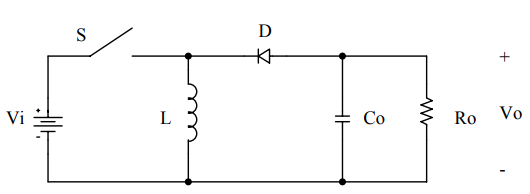
\includegraphics[scale=0.55]{imagens/circuito_buck_boost.png}
\caption{Circuito do conversor Buck-Boost.}\label{cbobu} 
\caption*{Fonte: Introdução aos conversores CC-CC (2001)}
\end{figure}

Durante a etapa de condução da chave $S$, a fonte fornece energia para o indutor $L$, enquanto o capacitor $C_o$ descarrega sobre o resistor $R_o$. Após a abertura da chave $S$, o indutor alimenta tanto o capacitor quanto a resistência, mas de forma invertida à fonte. A figura \ref{g1bobu} ilustra a tensão no indutor $L$.

\begin{figure}[h]
\center
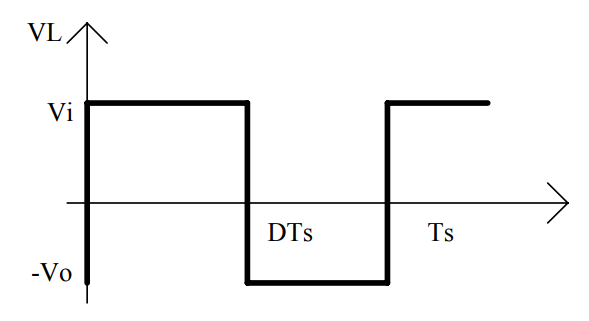
\includegraphics[scale=0.55]{imagens/grafico1_buck_boost.png}
\caption{Comportamento da tensão no indutor $L$ de um conversor Buck-Boost.}\label{g1bobu} 
\caption*{Fonte: Introdução aos conversores CC-CC (2001)}
\end{figure}

Considerando a tensão média no indutor nula, segue que \[
    \frac{1}{T_{s}}\int_{o}^{DT_{s}}V_{i}dt =  \frac{1}{T_{s}}\int_{o}^{(1-D)T_{s}}(V_{o} - V_{i})dt
\] \[
\implies\frac{V{o}}{V{i}} = \frac{D}{1-D}
.\] Logo, é fácil ver que o conversor pode tanto abaixar quanto elevar a tensão de forma contínua a partir da razão cíclica. A figura \ref{g2bobu} ilustra essa relação.

\begin{figure}[h]
\center
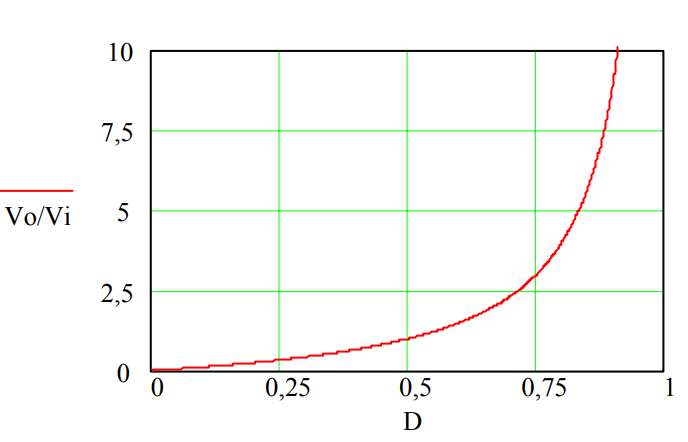
\includegraphics[scale=0.55]{imagens/grafico2_buck_boost.png}
\caption{Relação entre o ganho estático de um conversor Buck-Boost e a razão cíclica do chaveamento.}\label{g2bobu} 
\caption*{Fonte: Introdução aos conversores CC-CC (2001)}
\end{figure}

O comportamento da tensão e da corrente nos diversos componentes desse conversor está ilustrado na figura \ref{g2bobu}.

\begin{figure}[h]
\center
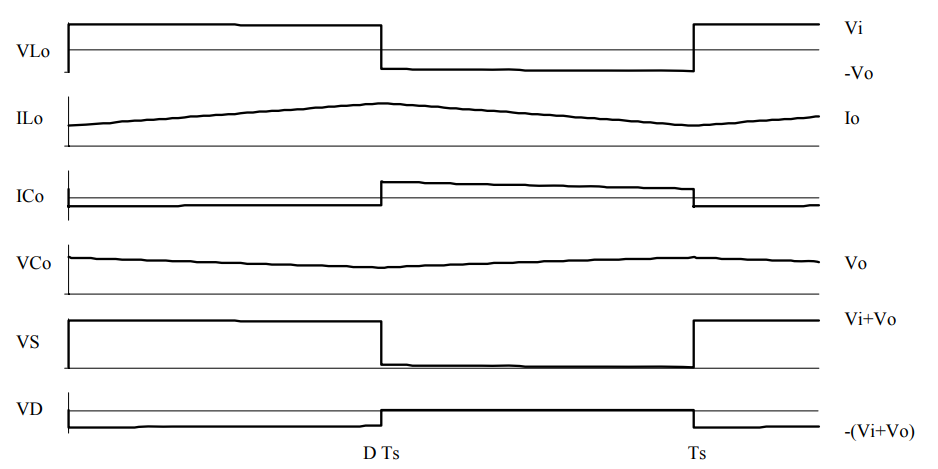
\includegraphics[scale=0.55]{imagens/grafico3_buck_boost.png}
\caption{Comportamento da tensão e da corrente nos diversos componentes de um conversor Buck-Boost.}\label{g3bobu} 
\caption*{Fonte: Introdução aos conversores CC-CC (2001)}
\end{figure}

Dessa forma, o conversor Buck-Boost fornece uma implementação que abaixa e eleva a tensão de forma contínua, mas distorce a corrente tanto para a alimentação quanto para a carga.

